Juana arma triángulos con fósforos. Arma figuras que guardan una relación en particular. Observa la siguiente imagen:

\begin{minipage}{0.4\linewidth}
    \begin{figure}[H]
        \centering
        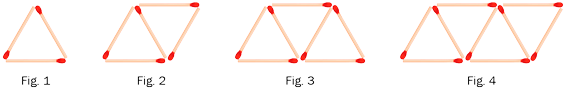
\includegraphics[width=0.9\linewidth]{../images/c9b918ae22f368bf3b8bbb644dfd20d4530338f0}
        \caption{Brocheta demostrativa}
        \label{fig:c9b918ae22f368bf3b8bbb644dfd20d4530338f0}
    \end{figure}
\end{minipage}\hfill
\begin{minipage}{0.6\linewidth}
    Juana sigue armando triángulos según la secuencia de la imagen.
    Cuando termine de armar la Figura \ref{fig:c9b918ae22f368bf3b8bbb644dfd20d4530338f0},
    \textbf{¿cuántos fósforos habrá usado en total?}

    \begin{solutionbox}{1.2cm}
        255 fósforos.
    \end{solutionbox}
\end{minipage}